\chapter{Processamento de Linguagem Natural}
\label{chapter:nlp}

Neste capitulo serão apresentadas as técnicas de Processamento de Linguagem
Natural que compõe um classificador, como o de análise de sentimento.
De modo geral, esse processo é composto de 3 etapas, como demostrado no
diagrama~\ref{fig:nlp_diagram}.
As seções a seguir descrevem cada uma destas fases.

\begin{figure}[h]
\begin{center} {
    \begin{center}
    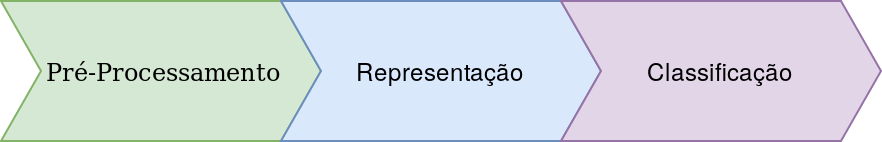
\includegraphics[scale=0.35]{images/nlp_diagram.png}
    \caption{Etapas de algoritmos de Processamento de Linguagem Natural.}
    \label{fig:nlp_diagram}
    \end{center}
}
\end{center}
\end{figure}

\section{Pré-Processamentos}

A primeira etapa aplicada para elaboração de modelos de NLP é o
pré-processamento.
Esta fase consiste na limpeza e preparação dos dados, visando melhorar a
performance do classificador seja retirando ruídos dos textos, reduzindo o
tamanho do vocabulário ou formatando o texto de maneira a facilitar a modelagem.
O volume do vocabulário considerado é costuma ser limitado seja pelos recursos
computacionais quanto pelo requisito mínimo de estatística das palavras na base
de dados.
Portanto, técnicas de pré-processamento que reduzam o tamanho total do
vocabulário tem um importante papel na garantia de bom funcionamento dos
classificadores.

Como a maior parte dos modelos de NLP trabalham a nível de palavra é necessário
separar separar o documento em frases, com algoritmos como o Punkt~\cite{kiss06},
e posteriormente, em palavras.
Esse processo chamado \textit{tokenização} precisa ser robustos a abreviações,
números e características do idioma ao qual será aplicado, como contração de
palavras.
Se tratando de redes sociais, também é relevante tratar os links, as
\textit{hashtags} e as menções a usuários.

Algoritmos de correção ortográfica~\cite{damerau64}\cite{navarro01} podem ser
eficientes para aprimorar a qualidade dos textos, principalmente se tratando de
meios de comunicação dinâmicos como as redes sociais.

Técnicas de stemização consistem na extração do o radical das palavras,
como o obtido pelo algoritmo de Porter~\cite{porter80}, um exemplo é dado com a
palavra "montanha" que possuí radical "mont", o mesmo obtido pela palavra
"monte".
Por outro lado, o processos de lematização tem finalidade parecida, porém
transforma a palavra em sua forma base, forma como elas aparecem no dicionario,
podendo então diferenciar palavras com o mesmo radical, como "banco" e "bancários".
Ambas as técnicas visam tornar as etapas posteriores menos sensíveis a flexões
gramaticais, além de colaborar na redução do vocabulário.

Uma das principais etapas do pré-processamento é a remoção das
\textit{stopwords}, conjunto de palavras que informação pouco discriminante
para uma dada aplicação~\cite{lo05}, geralmente são compostas pelas palavras
mais comuns da língua, principalmente artigos e preposições.
O objetivo da remoção das \textit{stopwords} é diminuir ruídos dos dados
textuais, assim simplificando a etapa de modelagem.
\citet{saif14} fizeram um estudo comparando diversos métodos de seleção de
\textit{stopwords} e o impacto das mesmas na classificação de sentimento de
\textit{tweets}.
A identificação de classe gramatical, em inglês \textit{part of speech}, além de
ser tipicamente utilizada como entrada de modelos de NLP, também pode ser útil
para selecionar \textit{stopwords}.

\section{Representações}

Uma vez que os tratamentos iniciais dos textos são feitos chega-se a etapa de
preparar esses dados para serem processados pelo modelo.
Para isso, os documentos são transformados de sequências de palavras em vetores
ou matrizes.
Há diversas técnicas desenvolvidas com essa finalidade, estas podem ser
divididas em representações esparsas e representações densas.
As representações esparsas são as mais simples de serem aplicadas dado que, em
geral, não dependem do treinamento de nenhum modelo.
Entretanto, as representações esparsas resultam em vetores ou matrizes de
dimensão na ordem de, pelo menos, o tamanho do vocabulário escolhido, como os
vocabulários costumam ser muito extensos (centenas de milhares de palavras em
alguns casos) o tamanho e a esparsidade da representação obtida podem dificultar
o treinamento dos classificadores.
Para contornar essa dificuldade foram criados algoritmos de representações
densas.
Por transformarem os documentos em vetores ou matrizes de baixa dimensão estes
algoritmos foram os responsáveis pela viabilidade de utilização de técnicas de
\textit{Deep Learning} aplicadas ao processamento de linguagem natural.
Nessa seção descreveremos algumas das principais técnicas de representação de
texto.

\subsection{Codificação One-Hot}

A codificação \textit{One-Hot} representa cada palavra de maneira maximamente
esparsa.
Para tal, é definido um espaço vetorial em que cada palavra do vocabulário
utilizado é equivalente a uma dimensão do espaço.
Portanto, um documento pode ser transcrito dessa forma em uma sequência de
vetores, ou matriz, em que cada palavra é um vetor com valor unitário na
dimensão da própria palavra e zero nas outras, como mostra a
Figura~\ref{fig:onehot}.

\begin{figure}[h]
\begin{center} {
    \begin{center}
    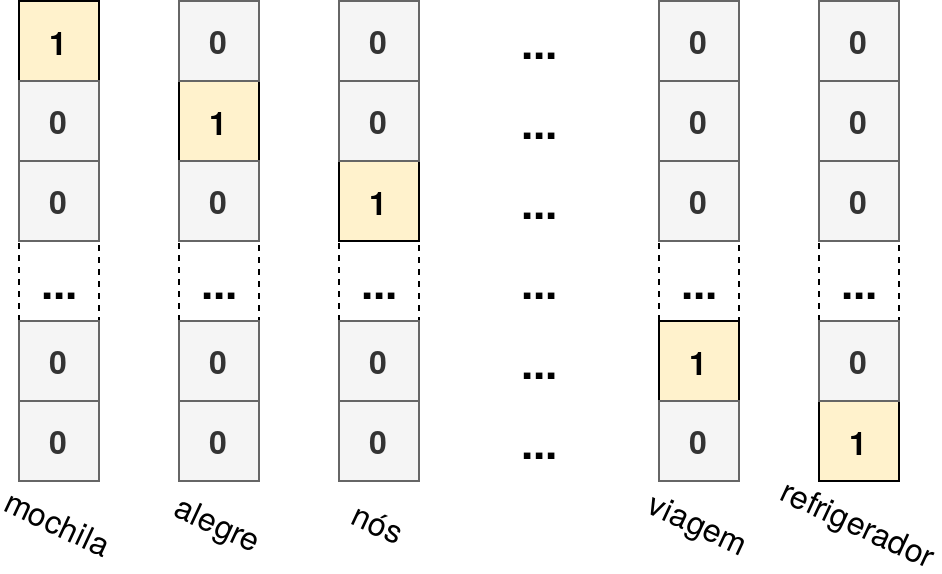
\includegraphics[scale=0.30]{images/onehot.png}
    \caption{Vetores \textit{One-Hot} de palavras de um dicionário.
             A dimensionalidade do vetor é igual ao tamanho do dicionário.}
    \label{fig:onehot}
    \end{center}
}
\end{center}
\end{figure}

Frequentemente encontramos nas línguas palavras compostas ou expressões.
Essas informações são perdidas na codificação \textit{One-Hot}.
Uma forma de se atenuar esse problema são com os chamados \textit{n-gramas}.
A ideia do \textit{n-grama} é formar tokens de 2, 3, ou \textit{n} palavras e
utiliza este conjunto de palavras como dimensão do espaço.
Entretanto, o aumento no número de palavras por token também gera um aumento
significativo do número de dimensões, dificultando o treinamento do
classificador.

\subsection{Bag-of-Words}

A codificação \textit{Bag-of-Words} é uma alternativa a representação de
mensagens como matrizes compostas de vetores \textit{One-Hot} de suas palavras.
Esta é feita pela soma destes mesmos vetores~\cite{manning10}.
Portanto, a representação final é dada por um único vetor, de tamanho
correspondente ao do vocabulário utilizado.
Esta técnica também tem a vantagem de transformar documentos de tamanho variados
em vetores de mesmas dimensões, fator que precisa ser contornado em codificações
baseadas em palavras.

\begin{figure}[h]
\begin{center} {
    \begin{center}
    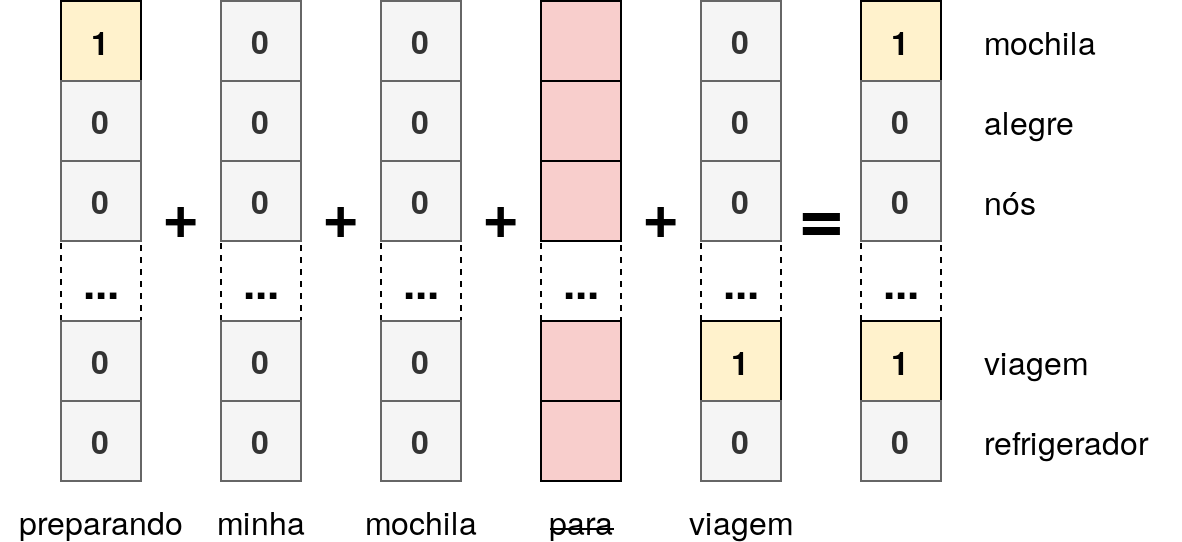
\includegraphics[scale=0.30]{images/bag_of_words.png}
    \caption{Processo de representação por \textit{Bag-of-Words} da frase
             ``Preparando minha mochila para viagem.''.
             A palavra ``para'' é removida durante o pré-processamento por
             ser uma \textit{stopword}.}
    \label{fig:bag_of_words}
    \end{center}
}
\end{center}
\end{figure}

Entretanto, visto que a distribuição de palavras em um corpus, em geral, segue a
lei de Zipf~\cite{powers98}, ou seja, sua frequência segue uma distribuição em
lei de potência.
Neste caso mesmo retirando \textit{stopwords}, as palavras mais comuns do
vocabulário ainda dominarão os documentos, e este comportamento pode ser
prejudicial para o treinamento dos modelos que serão menos expostos a palavras
incomuns.

% TODO: exemplo zipf grafico ou equacao

Para atenuar esse problema pode-se aplicar o \textit{term frequence-inverse
document frequence} (TF-IDF)~\cite{salton88}.
Neste caso, a representação segue a mesma estrutura proposta pela codificação
\textit{bag-of-words}, entretanto, cada palavra é ponderada por um multiplicador
inversamente proporcional a sua frequência nos documentos.

% TODO: equação tf-idf

\textit{Bag-of-words} e TF-IDF são métodos de representação muito presentes na
literatura pela sua simplicidade de implementação e pelos benefícios
anteriormente descritos, em especial em conjunto com modelos como a
SVM~\ref{sec:svm} que apresenta menos dificuldades de ser treinada em dados
esparsos.
Entretanto, um componente fundamental da linguagem é perdido nesse processo, o
contexto em que se insere cada palavra.
Pela representação agrupar todos os tokens em um único vetos a ordem das
palavras no documento é perdida, o que em muitos casos pode corresponder na
inviabilidade de uma classificação precisa do mesmo.

% TODO: talvez mostrar exemplo em que a ordem faria diferença

As técnicas de representações densas que serão apresentadas a seguir além de
resolverem o obstáculo da dimensionalidade dos dados também viabilizam a
classificação por modelos que levem em conta o contexto de cada palavra.

\subsection{Word2Vec} \label{sec:w2v}

\textit{Word2Vec}~\cite{mikolov13} foi uma das primeiras técnicas de
representação densa de palavras amplamente adota pela indústria e academia.
Representações densas são aquelas em que cada palavra é transformada em um vetor
de números reais de baixa dimensionalidade, tipicamente dezenas ou poucas
centenas de dimensões.
\citet{mikolov13} mostraram que essa representação é capaz de capturar parte dos
sentidos semânticos e sintáticos das palavras, aproximando as que são sinônimas
ou exerçam a mesma função gramatical, atenuando assim o problema da disparidade
de frequência das palavras.

Esta técnica é um modelo constituído de uma rede neural de uma camada escondida.
Para o treinamento do mesmo são feitas janelas de um número arbitrário de
palavras que servirão como entrada do modelo.
Dessas janelas há duas variações: o \textit{continuous bag-of-words} em que
o modelo é treinado para prever a palavra central da janela de entrada a partir
das outras palavras da janela, ou o \textit{skipgram} que a partir da palavra
central da treina-se para prever o seu contexto.
A Figura~\ref{fig:w2v} ilustra a diferença entre os treinamentos.
As entradas e saídas do modelo são representadas pela codificação
\textit{one-hot} dos termos.
A quantidade de neurônios escolhido para a camada escondida da rede resultará na
dimensionalidade da representação.
A representação das palavras serão os pesos da camada de entrada do modelo
treinado.

\begin{figure}%
    \centering
    \subfloat[Continuos Bag-of-Word]{{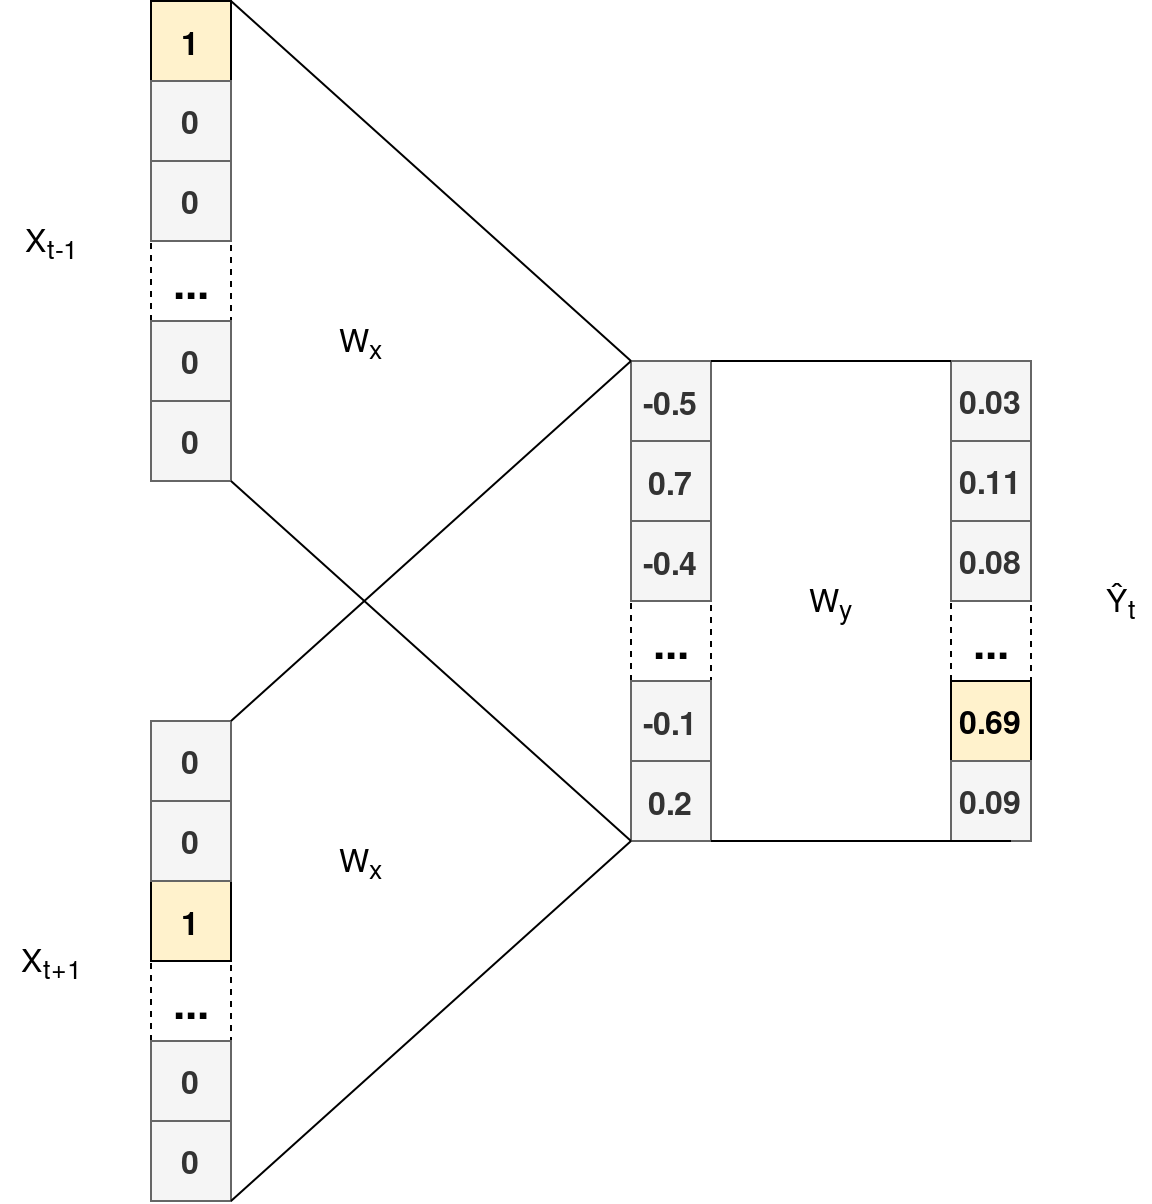
\includegraphics[scale=0.25]{images/word2vec_cbow.png}}}%
    \qquad
    \subfloat[Skipgram]{{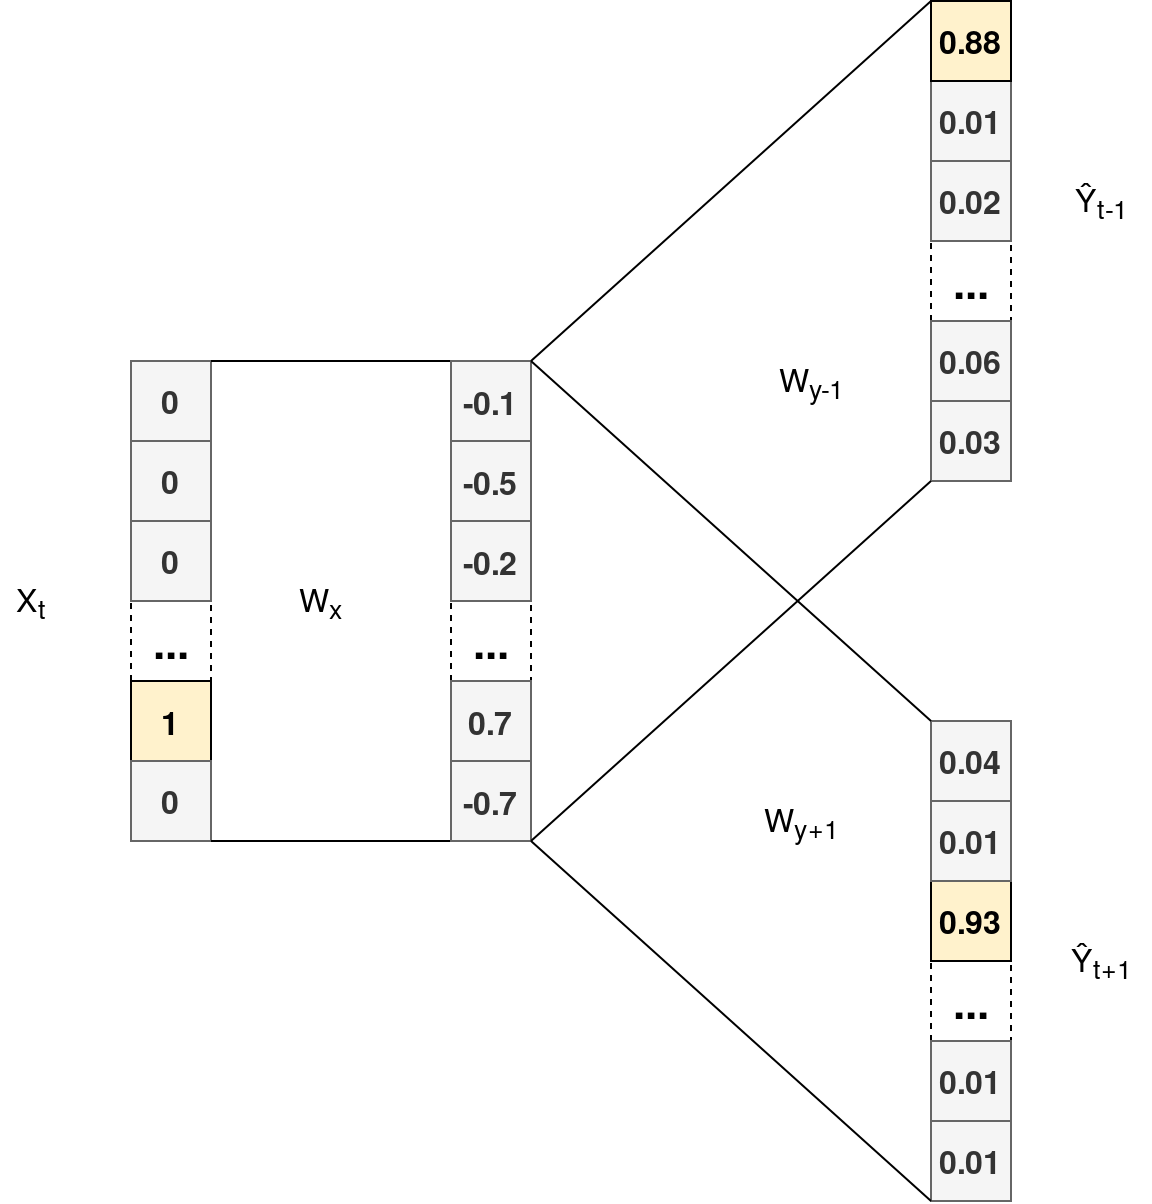
\includegraphics[scale=0.25]{images/word2vec_skip.png}}}%
    \caption{Esquemas de treinamento do Word2Vec. A matriz $X_t$ representa a
             palavra da janela na posição $t$ e $\hat{Y}_t$ a predição do modelo
             para a mesma, $W$, por sua vez, o conjunto de pesos treináveis.
             A representação resultante de uma palavra é dada pelo seu referente
             vetor na matriz de pesos de entrada $W_x$.}%
    \label{fig:w2v}%
\end{figure}

Apesar do \textit{Word2Vec} ser um modelo que precisa ser treinando, esse
treinamento é não-supervisionado dado que tanto as entradas quanto saídas do
modelo são obtidas diretamente dos documentos.
Desta forma, foi possível aplicar o algoritmo a grandes bases de dados
mineiradas da internet.
Esse alto volume de dados de treinamento foi essencial para que bons resultados
fossem alcançados.

Por ser a primeira representação densa de sucesso, o \textit{Word2Vec} foi
essencial para a aplicação de classificadores também baseados em redes neurais,
como os de \textit{Deep Learning} que obtiveram grande êxito em diversas
tarefas de processamento de linguagem natural.
Outras técnicas semelhantes e também amplamente adotadas na indústria foram
desenvolvidas neste mesmo período de tempo como o GloVe~\cite{pennington14} e
o FastText~\cite{bojanowski17}.

% TODO abrir matematica do W2V

\subsection{Representações por Redes Neurais Recorrentes}
\label{representation:rnn}

O sucesso do \textit{Word2Vec}, baseado em redes neurais \textit{feed forward}
inspirou a experimentação de outros tipos de redes neurais, dentre as quais as
redes neurais recorrentes e suas variações obtiveram bons resultados na
representação de palavras.
Nesta seção serão descritos alguns destes algoritmos.

A estrutura chamada \textit{Enconder-Decoder} desenvolvida por \citet{cho14} se
tornou a base das principais representações por redes recorrentes.
Esta estrutura consiste em uma rede neural recorrente divida em duas etapas: a
codificação, na qual uma sequência de tamanho variável é representada em um
vetor; e a decodificação em que este mesmo vetor é utilizado para obter uma
outra sequência de tamanho variável.
O \textit{Encoder-Decoder} é um modelo de aprendizado de sequências de tamanho
variável a partir de outra sequência de tamanho variável como entrada, em que
os tamanhos não necessariamente são os mesmos, reflexo do problema inicial em
que o mesmo foi desenvolvido para atacar, a tradução de textos.

\begin{figure}
\begin{center} {
    \begin{center}
    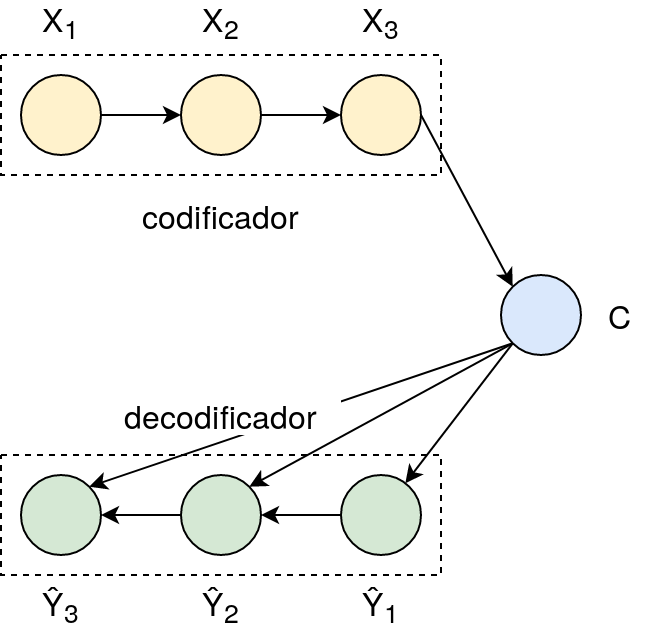
\includegraphics[scale=0.30]{images/encoder_decoder.png}
    \caption{Arquitetura Encoder-Decoder, constituída por duas camadas de redes
             recorrentes, a de codificação, e a de decodificação, ligadas por um
             conjunto de pesos $C$ que captura todo o contexto provindo da
             camada de codificação.}
    \label{fig:encoder_decoder}
    \end{center}
}
\end{center}
\end{figure}

Essa estrutura toda é treinada conjuntamente e pode ser utilizada para gerar
sequências de saída a partir de entradas ou avaliar um par de entrada e saída a
partir da probabilidade $p_{\mathbf{\theta}}(\mathbf{y} \mid \mathbf{x})$
aprendida pelo treinamento, no qual $\mathbf{x}$ e $\mathbf{y}$ representam
respectivamente as sequências de entrada e saída e $\mathbf{\theta}$ o conjunto
de pesos do modelo treinado.

A etapa de codificação desse modelo pode ser vista como um resumo da sequência
de entrada em um vetor de tamanho fixo, assim sendo, o mesmo pode ser utilizado
para representações de documentos, ou palavras caso aplicada sequência de
tamanho unitário.
\citet{cho14} demostram brevemente em seu trabalho que a codificação é capaz de
capturar significados semânticos e sintático das palavras.

\subsubsection{ELMo}
% Deep contextualized word representations

ELMo~\cite{peters18}, sigla para \textit{Embeddings from Language Models}, em
português Representações para Modelos Linguísticos, se diferencia do modelo de
\citet{cho14} por levar em consideração o contexto de uma dada palavra para
obter sua representação, inspirado por \citet{peters17} e \citet{mccann17}.
Isto é, uma palavra que possua múltiplos sentidos terá representações diferentes
dependendo da frase em que está inserida.
O modelo é composto de uma rede LSTM~\cite{hochreiter97} bi-direcional
multicamada, treinada de maneira não supervisionada a partir do objetivo de
prever a palavra seguinte.

Estudos anteriores mostram que em modelos de redes recorrentes multicamadas,
a melhor camada escolhida para representação das palavras depende da finalidade
em que se deseja aplicá-la
~\cite{hashimoto16}~\cite{sogaard16}~\cite{belinkov17}~\cite{melamud16}, e que
em geral, camadas inferiores codificam melhor informação sintética e camadas
superiores a informação semântica.
A proposta de ELMo é para cada tarefa treinar uma combinação linear das
representações obtida por cada camada da rede.

% TODO: diagrama (ver http://jalammar.github.io/illustrated-bert/)

\citet{peters18} mostram que ELMo foi capaz de obter resultados melhores que o
estado da arte em diversas tarefas do processamento de linguagem natural.
Além de capturar informação sintética e semântica, ELMo se mostrou capaz de
desambiguar o contexto de palavras, problema até então não resolvido pelos
principais algoritmos de representação.

\subsection{BERT}
% bert - 2018 - BERT: Pre-training of Deep Bidirectional Transformers for Language Understanding

Outra técnica de representação bastante utilizada atualmente para representação
de palavras é a BERT~\cite{devlin18}, \textit{Bidirectional Transformers}, mas
antes de explicá-la será apresentada abaixo a arquitetura Transformers em que a
mesma se baseia.

\subsubsection{Transformers}
% transformers - 2017 - Attention is all you need (boa explicacao dos conceitos)

Um dos principais problemas de redes neurais recorrentes é o "esquecimento".
O esquecimento é observado quando ao tentar prever uma palavra no final de uma
longa sequência se perde influência das primeiras palavras da mesma por causa da
sucessivas multiplicações dos pesos entre ambas.
Apesar do algoritmo LSTM~\cite{hochreiter97}, \textit{Long-Short Term Memory},
que visa atenuar esse efeito criando um peso adicional, chamado de portão, que
controla o quanto os pesos de contexto são atualizados entre cada iteração de
palavras de uma sequência, o esquecimento continua sendo um fator limitante.

O mecanismo de atenção desenvolvido por \citet{bahdanau14} também tem como
objetivo diminuir o efeito do esquecimento.
Este consiste em um conjunto de pesos adicionais que multiplicados pelos pesos
de estados das iterações anteriores formam os pesos de estado da iteração
corrente, como também descrito em mais detalhes por \citet{luong15}.
A atenção se tornou uma das principais adições feitas a redes recorrentes
aplicadas a processamento de linguagem natural.

Inspirado nesse mecanismo, \citet{vaswani17} propuseram a arquitetura
Transformer para tradução de textos.
Essa arquitetura consiste em um sistema de \textit{Encoder-Decoder} desta vez
composto por redes neurais \textit{feed forward} multi camadas em que a
dependência temporal entre as palavras de um documento é atacada apenas pelo
sistema de \textit{self-attention}, ou, atenção própria.

Enquanto o mecanismo de atenção é composto se dá por um único conjunto de pesos,
a \textit{self-attention} é dividido em 3: os pesos de busca, de resposta e de
valor.
Cada palavra do vocabulário terá um de cada vetor associado a mesma que será
treinado em conjunto com o resto da arquitetura.
Para cada palavra do documento será feito um produto interno do seu vetor de
busca e os vetores de resposta das outras palavras da sentença, resultando em um
valor único de atenção entre cada par possível de palavras de uma sentença.
Após calcular esse valor será realizado uma operação de Softmax para que a norma
do vetor de atenção seja unitária.
Posteriormente se multiplica o vetor resultante pelo vetor de valor da palavra
de resposta, essa operação tem a finalidade de diminuir a importância de
palavras sem potencial discriminatório, como as \textit{stopwords}.
Assim são calculadas as entradas da rede \textit{feed forward}.

% TODO: figura exemplificando processo http://jalammar.github.io/illustrated-transformer/

% TODO: figura com o resultado http://jalammar.github.io/images/t/transformer_self-attention_visualization.png
% pode ser print do tensor2tensor

A etapa de codificação do Transformer é composta por uma cascata de unidades
formadas por uma camada de \textit{self-attention} seguida de uma camada de
rede \textit{feed forward}.
Diferentemente das redes recorrentes, o Transformer requer um tamanho fixo de
entrada, sendo um parâmetro a ser definido a depender da base de treinamento
escolhida.
Apesar das redes \textit{feed forward} não possuírem um conceito de sequência
assim como as redes recorrentes, essa arquitetura provou ser eficiente em
tarefas de processamento de linguagem natural ao mesmo tempo que possuem
treinamento significativamente menos custosos que a mesma~\cite{vaswani17}.

\subsubsection{Arquitetura BERT}

O sucesso do Transformer em traduções inspirou sua aplicação em outras tarefas.
\citet{radford18} propuseram utilizar apenas a camada de decodificação do
Transformer junto com uma adaptação da sequência de entrada para adequar a
tarefa a ser realizada.
O modelo é pré-treinado com uma quantidade massiva de dados na predição da
palavra seguinte e posteriormente é feito um ajuste fino com uma base de dados
da tarefa desejada.
Esta nova arquitetura foi capaz propagar os ganhos de performance do Transformer
para toda gama de tarefas de NLP.

Entretanto, tanto o Transformer original quanto o de \citet{radford18} são
modelos unidirecionais, prevendo a palavra, ou sentença à direita a partir do
contexto à esquerda.
\citet{devlin18} defendem que por serem unidirecionais os modelos restringem a
capacidade dos mesmos, principalmente em tarefas que utilizam a sentença
inteira, sendo a análise de sentimento um exemplo.
Proporam então um modelo bidirecional praticamente idêntico ao Transformer de
\citet{radford18} sendo sua única modificação ter o mecanismo de atenção
considerando o contexto bidirecionalmente.

Assim como o ELMo, o BERT pode ser usado diretamente como classificador além de
representar palavras.
\citet{devlin18} mostram as diferenças entre as camadas do modelo quando
utilizados como representação, assim como nas arquiteturas apresentadas
anteriormente as diferentes camadas possuem aprendizado de características
distintas da língua.

\section{Classificadores}

Nessa seção serão abordadas as diferentes estratégias para classificação de
sentimento.
As etapas descritas anteriormente lidam com a preparação dos documentos para
realização da classificação, apesar da complexidade dos métodos apresentados os
classificadores podem ser tão simples quanto contadores de palavras positivas e
negativas.
Podemos dividi-los em algoritmos baseados em dicionário e algoritmos de
aprendizado de máquina~\cite{taboada11}, suas características serão descritas
abaixo.

\subsection{Baseados em Dicionário} \label{sec:dictionary}

Uma das técnicas mais simples para classificação de sentimento é feita a partir
da elaboração de um dicionário composto por palavras que tenham conotação
positiva ou negativa.
A formação de um dicionário de sentimento pode ser feita de forma
manual~\cite{stone66}~\cite{tong01} ou de forma automática.
Dentre as maneiras automáticas temos a aplicado por \citet{hu04} que é feito a
partir de um conjunto inicial de palavra anotadas e de um dicionário de
sinônimos e antônimos tal qual o WordNet~\cite{miller90}.
Um exemplo é selecionar as palavras semente ``bom'' e ``ruim'' e montar uma base de
palavras recursivamente a partir dos seus sinônimos e antônimos.
Formas similares de identificação de palavras com sentimento baseados em
dicionários e palavras semente foram desenvolvidas por \citet{blair08},
\citet{rao09}, \citet{hassan10}, entre outros.

Existindo um dicionário, a classificação de polaridade de um documento é dada
com a partir de alguma função dos sentimentos das palavras que o compõem.
É comum a inclusão algumas características sintáticas como identificação de
adjetivos intensificadores e identificação de negação para ponderar a pontuação
de sentimento de uma palavra ou expressão~\cite{taboada11}.
A função de classificação pode ser tão simples quanto uma média do sentimento
das palavras ou, por exemplo, um calculo de proximidade entre o conjunto de
palavras do documento e as palavras ``excelente'' e ``ruim'', representando as
classes positivas e negativas, como propõe \citet{turney02}.

% pang and lee 2008 4.5.1
% Lexicon-Based Methods for Sentiment Analysis
% Liu 2012 sentiment analysis
% Mining and Summarizing Customer Reviews tem boas referencias no 2.2

\subsection{Modelos Lineares}

Naturalmente, as primeiras aplicações de aprendizado de máquina em análise de
sentimento fizeram uso de modelos simples, como os modelos lineares.
\citet{pang02} fizeram um dos primeiros estudos comparativos entre estes
métodos.
A seguir, serão descritos os dois principais modelos lineares utilizados em
processamento de linguagem natural: Naïve Bayes e Máquina de Vetor de Suporte.

\subsubsection{Naïve Bayes}

O classificador de Naïve Bayes se baseia no teorema de Bayes \ref{eq:bayes} e
na premissa de independência entre as dimensões da representação dos dados.
Quando representamos um documento textual com, por exemplo, \textit{bag-of-words}
a premissa de independência significaria assumir que existe independência entre
as palavras do documento.
Apesar de não existir independência entre palavras na linguagem, este modelo foi
aplicado amplamente a tarefas de processamento de texto devido a sua performance
e simplicidade.

\begin{equation} \label{eq:bayes}
    P(A\mid B) = \frac{P(A) P(B \mid A)}{P(B)}
\end{equation}

\citet{schutze08} descreveram a formulação matemática desse modelo, como será
demostrado.
Será denominado $\mathbf{X}$ o corpus de treinamento e $\mathbf{x}$ um documento
desse corpus.
As classes que os documentos pertencem, como positivo e negativo, é chamada de
$c_k$, no qual $\mathbf{c}$ é o conjunto de classes.
Portanto, substituindo as variáveis da equação~\ref{eq:bayes} temos que a
probabilidade de um documento pertencer a uma determinada classe é dada por:

\begin{equation}
    p(c_k \mid \mathbf{x}) = \frac{p(c_k) \ p(\mathbf{x} \mid c_k)}{p(\mathbf{x})}
\end{equation}

Como se assume independência entre as variáveis temos que:

\begin{equation}
    p(x_i \mid x_{i+1}, \dots ,x_{n}, c_k ) = p(x_i \mid c_k)
\end{equation}

Logo, pode-se substituir $p(\mathbf{x} \mid c_k)$ pelo produtório de
$p(x_i \mid c_k)$:

\begin{equation}
    p(c_k \mid \mathbf{x}) = \frac{p(c_k) \prod_{i=1}^n p(x_i \mid c_k)}{p(\mathbf{x})}
\end{equation}

A probabilidade $p(\mathbf{x})$ será constante, logo não influenciará o
treinamento, portanto temos que a relação entre a probabilidade de um documento
pertencer a classe é dada por:

\begin{equation}
    p(c_k \mid \mathbf{x}) \propto p(c_k) \prod_{i=1}^n p(x_i \mid c_k)
\end{equation}

Sendo assim, a tarefa da classificação que é encontrar a classe de maior
probabilidade.

\begin{equation}
    \hat{y} = \operatorname{max} p(c_k \mid \mathbf{x}) = \underset{k \in \{1, \dots, K\}}{\operatorname{max}} \ p(c_k) \displaystyle\prod_{i=1}^n p(x_i \mid c_k)
\end{equation}

A dependência entre a predição e o conjunto de treino então é dada por $p(c_k)$
e $p(\mathbf{x} \mid c_k)$, esses valores são obtidos por máxima verossimilhança.
O parâmetro $p(c_k)$ é dado pela proporção de vezes que a classe aparece no
conjunto de treino.
Tendo o conjunto de treino o tamanho $m$ de documentos:

\begin{equation}
    \hat{p}(c_k) = \frac{\sum_{i=1}^m [y_i = c_k]}{m}
\end{equation}

Por sua vez, $p(x_r \mid c_k)$ é estimado pela proporção entre uma determinada
característica $x_r$ com o total de de características do subconjunto de dados
$\mathbf{X_{c_k}}$ pertencentes a classe $c_k$:

\begin{equation}
    \hat{p}(x_r \mid c_k) = \frac{\sum_{j=i}^{m'} \sum_{i=1}^n [x_{ji} = x_r]}{|\mathbf{X_{c_k}}|}
\end{equation}

O Naïve Bayes pode ser aplicado tanto a vetores inteiros da representação
\textit{bag-of-words} de frequência de palavras em um documento quanto pelo seu
equivalente binário que assinala presença ou não de uma determinada palavra.
Ao considerar a frequência de palavras aplicamos o modelo multinomial enquanto
ao utilizar a representação de forma binária temos o modelo de Bernoulli.
O modelo de Bernoulli é mais eficiente para documentos e vocabulários pequenos
enquanto o multimodal se sobressaí no caso oposto~\cite{schutze08}.

Apesar da premissa de independência não ser verdadeira para língua, e não ser um
bom estimador~\cite{schutze08}, Naïve Bayes se mostra eficiente na
classificação, em especial quando existe um conjunto de características de
semelhante importância.
Sua principal vantagem se dá pelo baixo custo computacional de treinamento visto
que seus parâmetros são estimados apenas por contagens na base de dados.

\subsubsection{Máquina de Vetor de Suporte}
\label{sec:svm}

A Máquina de Vetor de Suporte, também chamada de SVM, é um algoritmo que busca
encontrar um vetor que melhor separe duas classes.
A diferença entre esse algoritmo e outros classificadores como a regressão
linear é que o SVM tem objetivo de obter o vetor que maximize a distância entre
as margens das classes, enquanto a regressão linear, em geral, minimiza uma
função custo baseada na distância entre o centro de massa das classes.

\begin{figure}
\begin{center} {
    \begin{center}
    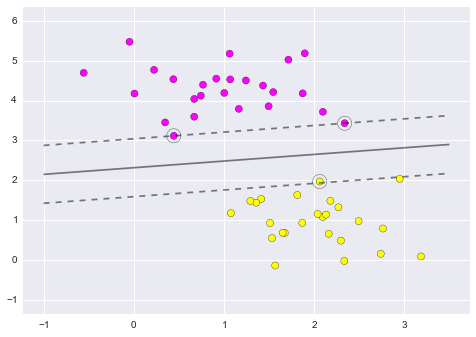
\includegraphics[scale=0.6]{images/svm.png}
    \caption{SVM classificando duas classes linearmente separáveis.}
    \small Imagem com direitos cedidos para uso não comercial, retirada de~\cite{vanderplas15}
    \label{fig:svm}
    \end{center}
}
\end{center}
\end{figure}

Entretanto, por se basear na margem das classes, o SVM não é capaz de separar
classes que tenham sobreposição.
Como forma de contornar esse problema foi criada uma variável de relaxamento de
forma a controlar o quanto de sobreposição é permitido entre as classes como
explicam \citet{cortes95}.
Ainda assim, até então a Máquina de Vetor de Suporte fica limitada a problemas
lineares.
Apenas com o desenvolvimento do chamado \textit{kernel trick} que o SVM pode ser
aplicável à problemas não-lineares e ganhou alta adoção.
O \textit{kernel trick} consiste em realizar uma transformação na representação
dos dados de forma que os mesmos sejam linearmente separáveis após a
transformação.
Mapeamentos radiais e polinomiais são dois dos exemplos de \textit{kernel}
amplamente utilizados.

Uma das principais propriedades do SVM é que seu treinamento independe da
dimensionalidade das características dos dados visto que seu aprendizado é feito
com base nas margens entre as classes.
Portanto, uma vez que os dados sejam separados por uma margem, mesmo que tenham
alta dimensionalidade, o vetor de suporte de classificação pode ser encontrado.
A aplicação de SVM para classificadores de texto foi proposta por
\citet{joachims98} visto que dados textuais representados por
\textit{bag-of-words} possuem 3 propriedades das quais se adéquam a
classificação por SVM:
\begin {enumerate*} [label=\itshape\alph*\upshape)]
    \item possuem alta dimensionalidade
    \item são esparsos
    \item tem poucas dimensões irrelevantes.
\end {enumerate*}
Apesar de \citet{joachims98} demostrar a efetividade do SVM para classificação
de texto utilizando \textit{kernels} não lineares, bons resultados são obtidos
mesmo sem a aplicação de \textit{kernel} como mostra \citet{pang02}.

\subsection{Modelos Não-Lineares}

Classificadores lineares a partir de representação por \textit{bag-of-words} ou
TF-DF dos textos foram o estado da arte em tarefas de processamento natural
durante os anos.
Entretanto, como visto anteriormente, ao aplicar técnicas como
\textit{bag-of-words} abre-se mão do contexto em que cada palavra aparece no
documento, este fator limita a performance da classificação.
Sem conseguir capturar o contexto essas técnicas se distanciam de como nós
interpretamos a língua.
Para diminuir essa lacuna, possibilitados pelo desenvolvimento de técnicas de
representações densas, passou a ser utilizados classificadores não-lineares que
visam adicionar alguma forma de contexto no processo.

\subsubsection{Deep Learning}

Dentre os modelos não-lineares os que mais se destacam em processamento de
linguagem natural são os de \textit{Deep Learning}, baseada em redes neurais.
Uma das principais características das redes neurais é que estas são algoritmos
capazes de aproximar qualquer função~\cite{hornik89}.
Com o desenvolvimento do método de treinamento por auto diferenciação, chamado
de \textit{backpropagation}, nos anos 80~\cite{werbos82} as redes neurais
foram amplamente adotadas.
Entretanto, dois principais fatores inviabilizaram o treinamento de redes
neurais de larga escala por muitos anos: o custo computacional do
\textit{backpropagation} e o efeito do \textit{vanishing gradient}~
\cite{hochreiter98}.
O \textit{vanishing gradient} é decorrente do efeito multiplicativo do
gradiente desde a camada de neurônios da saída até a camada de entrada.
O mesmo resulta em um treinamento menor da camada a medida que a mesma está
mais distantes da saída, estabelecendo assim uma dificuldade exponencial no
treinamento com relação ao número de camadas.

Com o desenvolvimento tecnológico e a elaboração de uma técnica de treinamento
camada-a-camada foi possível se sobrepor a esta barreira.
Este treinamento, proposto por \citet{hinton06}, em que cada camada de neurônio
é treinada individualmente e os valores obtidos por esse treinamento são
utilizados como inicialização do treinamento da rede completa.
Após esse trabalho começaram a testar redes neurais com um número cada vez
maior de camadas.
Denominou-se \textit{Deep Learning} a esse conjunto de modelos de redes neurais
profundas.

O salto de performance obtido pela aplicação de redes neurais
profundas~\cite{lecun15} em diversas áreas de conhecimento fez deste conjunto de
técnicas um objeto de estudo de muito interesse por pesquisadores e indústria.
Parte de seu sucesso se atribuí ao fato de que cada adicional na rede neural
permite que a mesma obtenha uma representação mais complexa dos dados.
Considerando o processamento de linguagem, diferentes tipos de redes neurais
foram testados para tentar capturar a complexidade desta informação,
com diferentes abordagens para adicionar o contexto em que cada palavra se
insere no processo de modelagem.
As seções abaixo descrevem os principais tipos de redes neurais aplicados a NLP.

% diferença principal de deep p tradicional é: contexto
% inspiração: http://dataskeptic.com/blog/episodes/2019/natural-language-processing

\subsubsection{Redes Neurais Convolucionais}

As redes convolucionais foram desenvolvidas prioritariamente para resolver
problemas como a classificação de imagens e reconhecimento de fala.
Um fator comum que essas tarefas compartilham é a possível translação da
informação.
Na classificação de imagens, por exemplo, um determinado objeto pode estar em
diferentes posições ou ocupar tamanhos distintos em diferentes imagem.
Apesar de ser possível aplicar redes neurais MLP ao problema, esta precisaria
aprender os mesmos padrões de neurônios em diferentes posições~\cite{lecun95}.
Além disso, neste tipo de problema existe uma característica da localidade da
informação, por exemplo, para reconhecimento de fala de uma palavra no final de
uma frase, a palavra imediatamente anterior é, em geral, mais importante que a
primeira palavra da mesma.
Ao se utilizar redes neurais MLP completamente conectadas entre camadas se
despreza essa propriedade, incorrendo em um maior custo computacional sem que
necessariamente se reflita em performance, ou pior, aumentando a chance de o
treinamento resultar em \textit{overfitting}.

A forma da rede convolucional atacar este problema da correlação espacial da
informação é utilizando filtros espaciais.
Cada camada da rede convolucional é formada por um conjunto de filtros que são
compostos por neurônios.
A iteração de treinamento da rede consiste no deslocamento de cada filtro por
toda dimensão da camada anterior.
Desta maneira os padrões locais são capturados por um mesmo filtro
independentemente de onde os padrões apareçam nos dados de entrada.
O deslocamento dos filtros durante o treinamento funciona como um
compartilhamento de pesos, reduzindo a quantidade de parâmetros livres da rede,
e assim sua probabilidade de \textit{overfitting}.

A interpretação de redes convolucionais aplicadas a processamento de texto não é
muito diferente de sua utilização com imagens.
Enquanto os filtros convolucionais exploram os padrões locais com filtros 2D de
poucos pixels em imagens, com o caso textual os filtros são unidimensionais e
percorrem a sequência de vetores de palavras com uma janela, capturando assim
parte do contexto em que cada palavra se insere.
Esse modelo já havia sido aplicado a documentos representados com
\textit{bag-of-words} como demostrado por \citet{kalchbrenner14} e
\citet{yih14} mas apenas quando utilizado em conjunto com a representação
Word2Vec como apresentou \citet{kim14} que esse algoritmo ganhou tração nas
tarefas de classificação de texto.
A disponibilidade de modelos Word2Vec pré-treinadas, somado a representação
densa que resulta em menor quantidade de parâmetros e menor probabilidade de
\textit{overfitting} torna essa combinação acessível para treinamento mesmo em
casos de grandes bases de dados, não obstante com performance superior como
mostra \citet{kim14}.

\subsubsection{Redes Neurais Recorrentes}

Outra forma de encapsular o contexto presente na linguagem é utilizando redes
neurais recorrentes.
As Redes Neurais Recorrentes são, em geral, treinadas com o algoritmo
\textit{Backpropagation Through Time}~\cite{williams95} (BPTT) em que a rede
recorrente se comporta como uma rede neural \textit{feedforward} na qual cada
camada representa um passo temporal nos dados de entrada, no caso de texto
podendo ser cada passo uma palavra.
Portanto, ao aplicar esse algoritmo sobre o texto, o contexto sequencial do
documento será capturado pela própria arquitetura da rede.

As variações de redes neurais recorrentes como apresentado em
\ref{representation:rnn} em grande parte também realizam classificação.
Um exemplo desta aplicação é mostrada por \citet{tai15} classificando sentimento
por uma rede LSTM.
Posteriormente, técnicas de classificação que misturam diferentes tipos de redes
foram testadas com êxito como mostram \citet{zhou16} em que a arquitetura é
constituída de uma camada de rede recorrente seguida por uma camada de rede
convolucional.

Apesar dos bons resultados obtidos nesses trabalhos, o treinamento por BPTT é
computacionalmente mais custoso que o \textit{backpropagation} de redes
\textit{feedforward} ou convolucionais, dado que o mesmo apresenta menos
oportunidade de paralelismo do treinamento.
Assim, esse algoritmo acaba sendo menos utilizado do que as redes
convolucionais, ou até mesmo os Transformers para classificação de documentos.

% JA EXPLICADO POR VOLTA DA PAGINA 9
%\subsection{Supervisão Distante}
%
%A boa performance dos algoritmos de Deep Learning depende da disponibilidade de
%grandes bases de dados de treinamento.
%Devido a grande disponibilidade de dados que tem processo de captação
%automatizados, como os de redes sociais, o fator limitante para desenvolvimento
%de bases de treinamento de grande volume passa a ser o processo de anotação
%manual da mesma.
%
%Uma das primeiras alternativa para formação automatizada de bases foi
%desenvolvida por \citet{craven99} que extraiu informações sobre relações entre
%proteínas a partir de um banco de dados textual de artigos biomédicos.
%Por não ser tão assertivo quanto a anotação manual, denomiram esse processo de
%anotação fraca.
%\citet{read05} se baseou nesse processo para criar a Supervisão Distante,
%técnica que consiste em utilizar uma característica dos dados que tenha
%correlação com as classes que se deseja modelar e utilizá-las como anotação.
%\citet{read05} utilizou emoticons
